% Maqueta del panel frontal del instrumento virtual (estilo LabVIEW)
\begin{tikzpicture}[font=\sffamily\scriptsize,
  ctrl/.style={draw=gray!60,fill=white,minimum width=1.55cm,minimum height=0.42cm,
     anchor=west,inner sep=2pt,align=right,text width=1.25cm}]
  % ventana
  \fill[gray!14,draw=gray!50,rounded corners=2pt] (0,0) rectangle (15.6,7.2);
  \fill[navy,rounded corners=2pt] (0,6.75) rectangle (15.6,7.2);
  \fill[navy] (0,6.75) rectangle (15.6,6.9);
  \node[white,anchor=west,font=\sffamily\scriptsize\bfseries] at (0.2,6.97)
    {Caracterizacion\_diodos.vi \ --- \ Panel frontal};
  \foreach \i in {0,1,2} \fill[white!80!navy] (15.3-\i*0.3,6.97) circle (0.07);
  % controles numéricos
  \newcommand{\control}[3]{%
    \node[anchor=south west,black!80] at (0.35,#1+0.42) {#2};
    \node[draw=gray!60,fill=gray!8,minimum width=0.28cm,minimum height=0.42cm,anchor=west,
      inner sep=0pt] (inc) at (0.35,#1+0.21) {};
    \fill[gray!55] ($(inc.center)+(-0.07,0.04)$) -- ++(0.14,0) -- ++(-0.07,0.09) -- cycle;
    \fill[gray!55] ($(inc.center)+(-0.07,-0.04)$) -- ++(0.14,0) -- ++(-0.07,-0.09) -- cycle;
    \node[ctrl] at (0.63,#1+0.21) {#3};}
  \control{5.45}{V start (V)}{$-$5,00}
  \control{4.35}{V end (V)}{5,00}
  \control{3.25}{\# muestras}{101}
  \control{2.15}{R (k$\Omega$)}{1,00}
  \node[anchor=south west,black!80] at (0.35,1.47) {Ruta del fichero};
  \node[draw=gray!60,fill=white,minimum width=2.9cm,minimum height=0.42cm,anchor=west,
     inner sep=2pt,text width=2.6cm] at (0.35,1.26) {\tiny C:\textbackslash Datos\textbackslash LED\_rojo.txt};
  \fill[Goldenrod!70] (3.1,1.12) rectangle ++(0.3,0.22);
  \fill[Goldenrod!90] (3.1,1.3) rectangle ++(0.13,0.06);
  % botón stop
  \node[draw=gray!60,fill=rojoaviso!80,text=white,rounded corners=1pt,minimum width=1.2cm,
    font=\sffamily\scriptsize\bfseries] at (1.2,0.5) {STOP};
  % imagen del circuito
  \node[draw=gray!50,fill=white,inner sep=3pt] at (5.0,3.6)
    {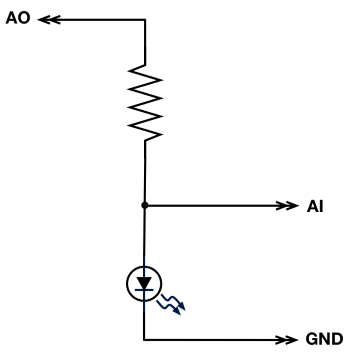
\includegraphics[height=4.4cm]{img/LED_cir.png}};
  \node[black!70] at (5.0,1.0) {LED\_cir.png};
  % gráfica XY
  \node[anchor=south west,black!80] at (8.0,6.2) {XY Graph};
  \begin{scope}[shift={(8.5,0.25)}]
  \begin{axis}[width=7.6cm,height=6.45cm,
    axis background/.style={fill=black!88},
    xmin=-5,xmax=2.5,ymin=-0.2,ymax=3.6,
    grid=major,grid style={green!35!black,line width=.3pt},
    xlabel={\sffamily VD (V)},ylabel={\sffamily ID (mA)},
    label style={font=\sffamily\scriptsize},
    tick label style={font=\sffamily\tiny},
    scaled y ticks=false,
    yticklabel={\pgfmathprintnumber[fixed,fixed zerofill,precision=1]{\tick}E+0},
    axis line style={gray},tick style={gray}]
    \addplot[white,mark=*,mark size=.8pt,thin] table[x=VD,y=ID]{datos/iv_rojo.dat};
  \end{axis}
  \end{scope}
\end{tikzpicture}
